\documentclass{article}
\usepackage{tikz}
\usepackage[paperheight=9in,paperwidth=20in,margin=0.4in,heightrounded]{geometry}
\definecolor{red}{RGB}{230,25,75}
\definecolor{green}{RGB}{60,180,75}
\definecolor{yellow}{RGB}{255,225,25}
\definecolor{blue}{RGB}{0,130,200}
\definecolor{orange}{RGB}{245,130,48}
\definecolor{purple}{RGB}{145,30,180}
\definecolor{cyan}{RGB}{70,240,240}
\definecolor{magenta}{RGB}{240,50,230}
\definecolor{lime}{RGB}{210,245,60}
\definecolor{pink}{RGB}{250,190,190}
\definecolor{teal}{RGB}{0,128,128}
\definecolor{lavender}{RGB}{230,190,255}
\definecolor{brown}{RGB}{170,110,40}
\definecolor{beige}{RGB}{255,250,200}
\definecolor{mint}{RGB}{170,255,195}
\definecolor{olive}{RGB}{128,128,0}
\definecolor{coral}{RGB}{255,215,180}

\usetikzlibrary{decorations.pathreplacing}
\begin{document}
\centering
\begin{minipage}{0.45\textwidth}
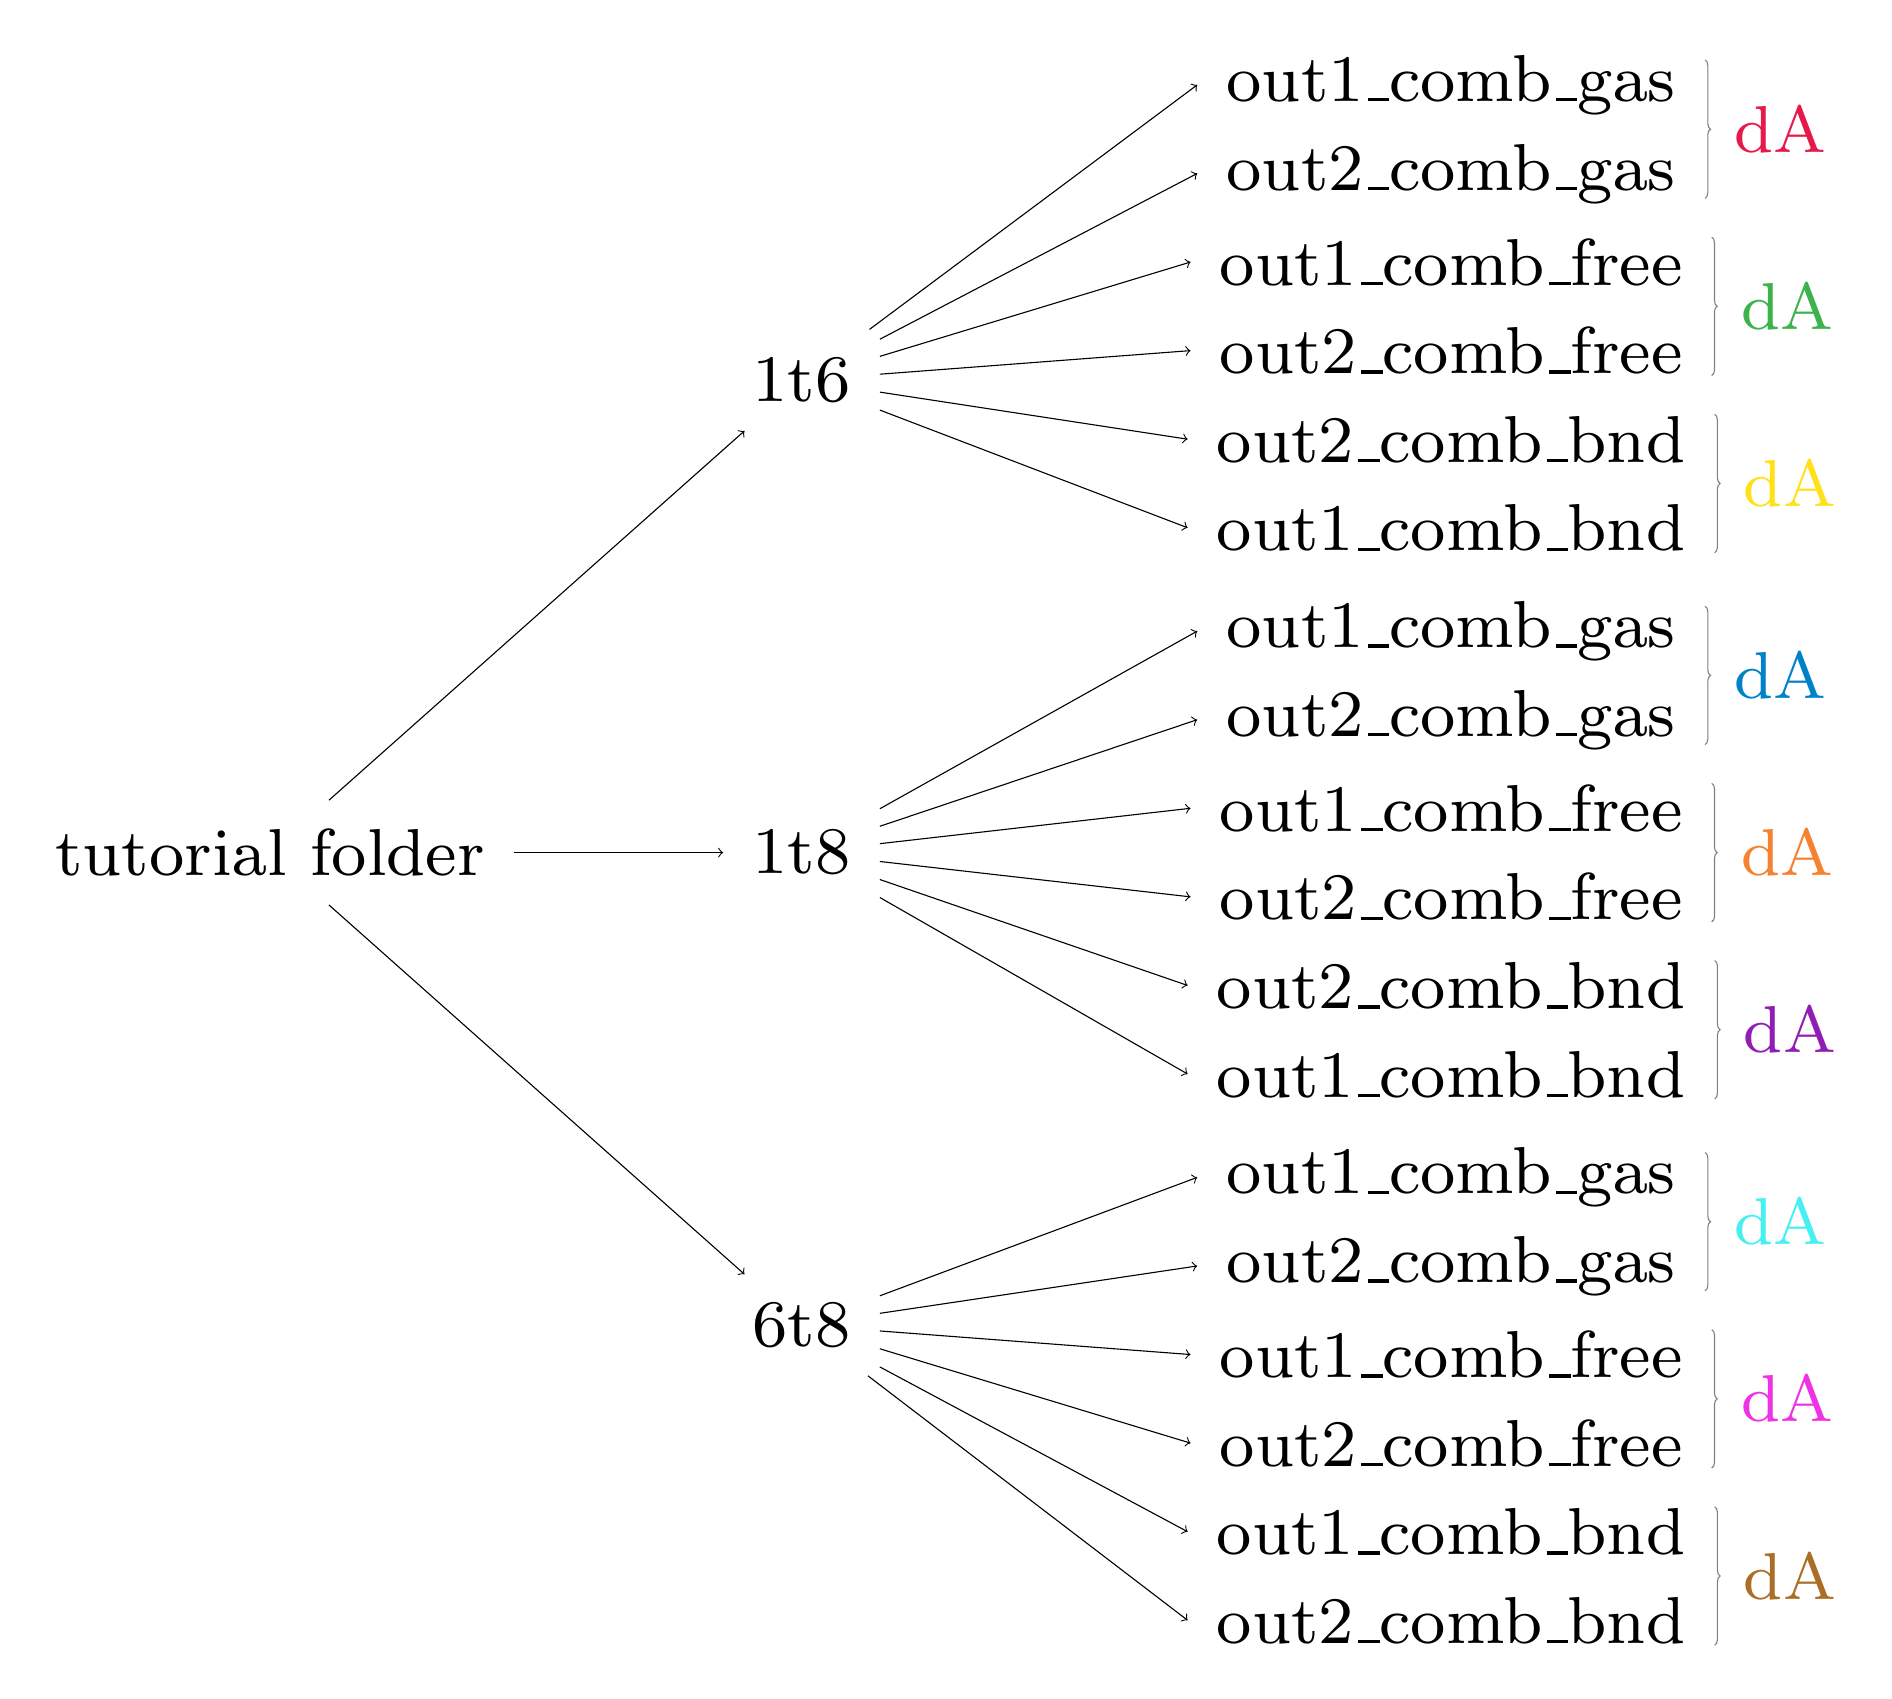
\begin{tikzpicture}[scale=3.0,transform shape,font=\footnotesize]
  \node (a) at (-1,0) {tutorial folder};
  \node (p1) at (1.25,2) {1t6};
  \node (p2) at (1.25,0) {1t8};
  \node (p3) at (1.25,-2) {6t8};

  \node (p1-g1) at (4.0,3.250) {out1\_comb\_gas};
  \node (p1-g2) at (4.0,2.875) {out2\_comb\_gas};
  \node (p1-f1) at (4.0,2.500) {out1\_comb\_free};
  \node (p1-f2) at (4.0,2.125) {out2\_comb\_free};
  \node (p1-b1) at (4.0,1.750) {out2\_comb\_bnd};
  \node (p1-b2) at (4.0,1.375) {out1\_comb\_bnd};
  \draw [gray,decorate,decoration={brace,amplitude=2pt}] ([yshift=3pt]p1-g1.east)  -- ([yshift=-3pt]p1-g2.east) 
   node [red,midway,right] {dA};
  \draw [gray,decorate,decoration={brace,amplitude=2pt}] ([yshift=3pt]p1-f1.east)  -- ([yshift=-3pt]p1-f2.east) 
   node [green,midway,right] {dA};
  \draw [gray,decorate,decoration={brace,amplitude=2pt}] ([yshift=3pt]p1-b1.east)  -- ([yshift=-3pt]p1-b2.east)
   node [yellow,midway,right] {dA};

  \node (p2-g1) at (4.0,0.9375) {out1\_comb\_gas};
  \node (p2-g2) at (4.0,0.5625) {out2\_comb\_gas};
  \node (p2-f1) at (4.0,0.1875) {out1\_comb\_free};
  \node (p2-f2) at (4.0,-0.1875) {out2\_comb\_free};
  \node (p2-b1) at (4.0,-0.5625) {out2\_comb\_bnd};
  \node (p2-b2) at (4.0,-0.9375) {out1\_comb\_bnd};
  \draw [gray,decorate,decoration={brace,amplitude=2pt}] ([yshift=3pt]p2-g1.east)  -- ([yshift=-3pt]p2-g2.east) 
   node [blue,midway,right] {dA};
  \draw [gray,decorate,decoration={brace,amplitude=2pt}] ([yshift=3pt]p2-f1.east)  -- ([yshift=-3pt]p2-f2.east) 
   node [orange,midway,right] {dA};
  \draw [gray,decorate,decoration={brace,amplitude=2pt}] ([yshift=3pt]p2-b1.east)  -- ([yshift=-3pt]p2-b2.east)
   node [purple,midway,right] {dA};

  \node (p3-g1) at (4.0,-1.375) {out1\_comb\_gas};
  \node (p3-g2) at (4.0,-1.750) {out2\_comb\_gas};
  \node (p3-f1) at (4.0,-2.125) {out1\_comb\_free};
  \node (p3-f2) at (4.0,-2.500) {out2\_comb\_free};
  \node (p3-b1) at (4.0,-2.875) {out1\_comb\_bnd};
  \node (p3-b2) at (4.0,-3.250) {out2\_comb\_bnd};
  \draw [gray,decorate,decoration={brace,amplitude=2pt}] ([yshift=3pt]p3-g1.east)  -- ([yshift=-3pt]p3-g2.east) 
   node [cyan,midway,right] {dA};
  \draw [gray,decorate,decoration={brace,amplitude=2pt}] ([yshift=3pt]p3-f1.east)  -- ([yshift=-3pt]p3-f2.east) 
   node [magenta,midway,right] {dA};
  \draw [gray,decorate,decoration={brace,amplitude=2pt}] ([yshift=3pt]p3-b1.east)  -- ([yshift=-3pt]p3-b2.east)
   node [brown,midway,right] {dA};

  \draw [->] (a) -- (p1);
  \draw [->] (a) -- (p2);
  \draw [->] (a) -- (p3);

  \draw [->] (p1) -- (p1-g1.west);
  \draw [->] (p1) -- (p1-g2.west);
  \draw [->] (p1) -- (p1-f1.west);
  \draw [->] (p1) -- (p1-f2.west);
  \draw [->] (p1) -- (p1-b1.west);
  \draw [->] (p1) -- (p1-b2.west);

  \draw [->] (p2) -- (p2-g1.west);
  \draw [->] (p2) -- (p2-g2.west);
  \draw [->] (p2) -- (p2-f1.west);
  \draw [->] (p2) -- (p2-f2.west);
  \draw [->] (p2) -- (p2-b1.west);
  \draw [->] (p2) -- (p2-b2.west);

  \draw [->] (p3) -- (p3-g1.west);
  \draw [->] (p3) -- (p3-g2.west);
  \draw [->] (p3) -- (p3-f1.west);
  \draw [->] (p3) -- (p3-f2.west);
  \draw [->] (p3) -- (p3-b1.west);
  \draw [->] (p3) -- (p3-b2.west);
\end{tikzpicture}
\end{minipage}
\hspace{5em}
\begin{minipage}{0.45\textwidth}

  \Huge
  \begin{tabular}{r r r r}
 &\multicolumn{1}{l}{dG gas} & \multicolumn{1}{l}{dG free} & \multicolumn{1}{l}{dG bound}\\
    1t6:&    \color{red} 31.882$+-$0.015&  \color{blue} 31.964$+-$0.263&   \color{cyan} 34.652$+-$0.069\\
    1t8:&  \color{green}-12.936$+-$0.018&\color{orange}-16.966$+-$0.048&\color{magenta}-14.336$+-$0.153\\
    6t8:& \color{yellow}-32.875$+-$0.019&\color{purple}-36.894$+-$0.002&   \color{brown}-37.570$+-$0.088\\
 Cycle Closure:&11.943$+-$0.030&12.035$+-$0.267&11.417$+-$0.189\\
\\
\\
 &\multicolumn{1}{l}{ddG Solvation}  & \multicolumn{1}{l}{ddG Binding}\\
     1t6:& 0.081$+-$0.263& 2.688$+-$0.272\\
     1t8:&-4.030$+-$0.051& 2.630$+-$0.160\\
     6t8:&-4.019$+-$0.019&-0.676$+-$0.088\\
 Cycle Closure:&0.092$+-$0.269&-0.618$+-$0.328
  \end{tabular}
\end{minipage}
\end{document}


%%% Local Variables:
%%% mode: latex
%%% TeX-master: t
%%% End:
